%%%%%%%%%%%%%%%%%%%%%%%%%%%%%%%%%%%%%%%%
%%%%%  xPhO LaTeX Beamer Template  %%%%%
%%%%%  Date: 17/03/2025            %%%%%
%%%%%  Authors:                    %%%%%
%%%%%       Nguyen Thanh Long      %%%%%
%%%%%       Nguyen Le Mai Huong    %%%%%
%%%%%       Nguyen Minh Phuong     %%%%%
%%%%%%%%%%%%%%%%%%%%%%%%%%%%%%%%%%%%%%%%

\documentclass[aspectratio=169, t]{beamer} % Ratio 16:9
\usepackage[T5]{fontenc}
\usepackage{lmodern}
\usepackage{graphicx} 
\usepackage{array}
\usepackage{longtable} % for long table

\usepackage{amsmath}

\usepackage{chngcntr}
\counterwithin{figure}{section}

\renewcommand{\familydefault}{\sfdefault} % Font

\usepackage{caption}
\usepackage{siunitx}

% \definecolor{BlueDefault}{rgb}{0.2,0.2,0.7}
\definecolor{BlueDefault}{RGB}{14,47,95}


% Hide navigation 
\setbeamertemplate{navigation symbols}{}

% Setup background
\newcommand{\normalbackground}{%
    \usebackgroundtemplate{
\includegraphics[width=\paperwidth,height=\paperheight]{Background/Normal_slide_xPhO.pdf}}%
}

\newcommand{\titlebackground}{%
    \usebackgroundtemplate{
\includegraphics[width=\paperwidth,height=\paperheight]{Background/Title_slide_xPhO.pdf}}%
}

% Change the title color to white
\setbeamercolor{frametitle}{fg=white} 

% push the title up by \raisebox
\setbeamertemplate{frametitle}{%
    \vspace{0.3em}
    \hspace{-1em} \insertframetitle
    % \vspace{2mm}
}

% Number of slide
\setbeamertemplate{footline}{%
    \hfill
    \insertframenumber/\inserttotalframenumber
    \hspace{7.5mm}
    \vspace{3.5mm}
}

%% Make Table of Contents %%
\AtBeginSection[]{
  \begin{frame}
  \frametitle{Mục lục}
  \tableofcontents[currentsection]
  \end{frame}
}

%% Section numbering %%
\setbeamertemplate{section in toc}[sections numbered]
\setbeamertemplate{subsection in toc}[subsections numbered]


\renewcommand{\figurename}{Hình}
\renewcommand{\tablename}{Bảng}


%%%%% Bibliography %%%%%
\usepackage[backend=biber,style=ieee]{biblatex}
\addbibresource{citation.bib}

\usepackage{url}
\usepackage{hyperref}
\hypersetup{
	colorlinks=true,
	linkcolor=BlueDefault,
	filecolor=BlueDefault,
    citecolor=BlueDefault,
	urlcolor=BlueDefault,
	pdftitle={Overleaf Example},
	pdfpagemode=FullScreen,
}

\begin{document}

\titlebackground

\begin{frame}[noframenumbering]
    \thispagestyle{empty}
    \bfseries
    \begin{flushleft}
        \vfill
        \vspace{5mm}
        \textcolor{BlueDefault}{\huge \bfseries Mô hình hóa và xử lý dữ liệu} \\
        \vspace{10mm}
        \textcolor{black}{\large \bfseries Người trình bày: Nguyễn Thành Long}
        \vfill
    \end{flushleft}
\end{frame}

\normalbackground

\section{Phân tích thứ nguyên}

\subsection{7 thứ nguyên}
\begin{frame}{7 Đại lượng SI và 7 thứ nguyên}
    \begin{table}
        \centering
        \begin{tabular}{|l|c|c|}
            \hline
            Đại lượng & Ký hiệu & Đơn vị \\
            \hline
            Chiều dài & \(L\) & Meter (m) \\
            \hline
            Khối lượng & \(M\) & Kilogram (kg) \\
            \hline
            Thời gian & \(T\) & Second (s) \\
            \hline
            Cường độ dòng điện & \(I\) & Ampere (A) \\
            \hline
            Nhiệt độ & \(\Theta\) & Kelvin (K) \\
            \hline
            Lượng chất & \(N\) & Mol (mol) \\
            \hline
            Cường độ sáng & \(J\) & Candela (cd) \\
            \hline
        \end{tabular}
        \caption{7 đại lượng cơ bản trong hệ SI và ký hiệu thứ nguyên tương ứng.}
    \end{table}
\end{frame}

\subsection{Phương pháp Rayleigh}
\begin{frame}{Phương pháp Rayleigh}
\vspace{-4mm}
\begin{columns}
\column{0.6\textwidth}

    \begin{itemize}
        \item \(\Delta t^\alpha m^\beta R^\gamma g^\delta \) là đại lượng không thứ nguyên.
    \end{itemize}
    \begin{equation}
        \left[ \Delta t^\alpha m^\beta R^\gamma g^\delta \right] = T^\alpha (M)^\beta (L)^{\gamma + \delta} (T^{-2})^\delta.
    \end{equation}
    nên
    \begin{equation}
        \left\{ \begin{array}{l}
            \alpha - 2\delta = 0 \\
            \beta = 0 \\
            \gamma + \delta = 0
        \end{array} \right.
        \rightarrowtail \left\{ \begin{array}{l}
            \alpha = 2\delta \\
            \beta = 0 \\
            \gamma = -\delta
        \end{array} \right.
    \end{equation}
    Chọn \(\delta = 1\) ta có
    \begin{equation}
        \Delta t = \sqrt{\frac{R}{g}} \ f(\theta).
    \end{equation}

\column{0.4\textwidth}
    \begin{figure}
        \centering
        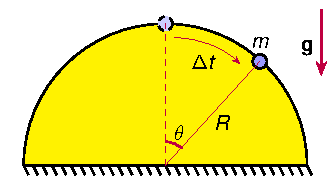
\includegraphics[width=0.9\textwidth]{Figures/Circle_sliding.pdf}
        \caption{Chất điểm trượt trên mặt tròn.}
    \end{figure}
\end{columns}

\end{frame}

\begin{frame}{Khi số biến lớn hơn số bậc tự do?}
\begin{columns}
\column{0.62\textwidth}
    \textbf{Bài toán dao động con lắc lò xo \cite{Lemons_2017}}
    \begin{equation}
        \left[ \omega m^\alpha k^\beta \rho^\gamma V^\delta g^\varepsilon \right]
        = T^{-1 - 2 \beta - 2 \varepsilon} M^{\alpha + \beta + \gamma} L^{3 \delta - 3 \gamma - \varepsilon}.
    \end{equation}
    Giải hệ phương trình và biểu diễn theo 2 biến tự do \(\delta, \varepsilon\):
    \begin{equation}
        \omega m^\alpha k^\beta \rho^\gamma V^\delta g^\varepsilon = \left( \frac{\omega m^{1/2}}{k^{1/2}} \right) \left( \frac{\rho V}{m} \right)^\delta \left( \frac{m^{4/3} g}{k \rho^{1/3}}\right)^\varepsilon.
    \end{equation}
    nên
    \begin{equation}
        \omega = \sqrt{\frac{k}{m}} \ f\left( \frac{\rho V}{m}, \frac{m^{4/3} g}{k \rho^{1/3}} \right).
    \end{equation}

\column{0.38\textwidth}
    \vspace{-8mm}
    \begin{figure}
        \centering
        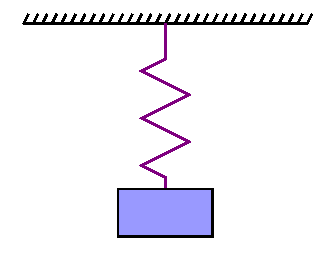
\includegraphics[width=0.9\textwidth]{Figures/Pendulum.pdf}
        \caption{Con lắc lò xo.}
    \end{figure}
    \vspace{-5mm}
    \begin{itemize}
        \item Khối lượng \(m\), độ cứng lò xo \(k\), khối lượng riêng của khí \(\rho\), thể tích chất lỏng \(V\), gia tốc trọng trường \(g\).
        \item Tần số \(\omega = f(m, k, \rho, V, g)\).
    \end{itemize}
\end{columns}
\end{frame}





\section{Machine learning và bài toán hồi quy}

\subsection{Bài toán hồi quy và hồi quy tuyến tính}

\begin{frame}{Bài toán hồi quy và hồi quy tuyến tính}
\begin{columns}
\column{0.4\textwidth}
    \vspace{-4mm}
    \begin{table}
        \centering
        \begin{tabular}{|c|c|c|c|}
            \hline
            \(x\) & \(y\) & \(x\) & \(y\) \\
            \hline
            1.01 & 1.45 & 10.97 & 6.53 \\
            2.04 & 2.03 & 11.94 & 6.98 \\
            2.98 & 2.47 & 12.98 & 7.53 \\
            3.95 & 3.01 & 13.95 & 8.00 \\
            5.01 & 3.49 & 15.01 & 8.50 \\
            5.99 & 4.02 & 15.99 & 8.93 \\
            7.02 & 4.47 & 17.02 & 9.49 \\
            7.98 & 4.95 & 18.07 & 10.02 \\
            9.03 & 5.52 & 19.06 & 10.52 \\
            10.01 & 6.02 & 19.91 & 11.03 \\
            \hline
        \end{tabular}
        \caption{Dữ liệu mẫu.}
    \end{table}

\column{0.6\textwidth}
    \begin{itemize}
        \item Bài toán: Tìm hàm \(f(x)\) sao cho \(y \approx f(x)\).
    \end{itemize}
    Dự đoán mô hình: \(f(x) = \beta_0 + \beta_1 x\).

    \begin{itemize}
        \item Tham số cần tìm: \(\boldsymbol{\theta} = (\beta_0, \beta_1)\).
        \item Hàm mất mát (Mean Squared Error):
        \[
        L(\boldsymbol{\theta}) = \frac{1}{N} \sum_{i=1}^{N} (y_i - f(x_i; \boldsymbol{\theta}))^2
        \]
        với \(N\) là số lượng mẫu dữ liệu.
        \item Mục tiêu: Tìm \(\boldsymbol{\theta}\) sao cho \(L(\boldsymbol{\theta})\) nhỏ nhất.
    \end{itemize}
\end{columns}
\end{frame}

\begin{frame}{Nghiệm của hồi quy tuyến tính}

\begin{columns}
\column{0.5\textwidth}
    \begin{itemize}
        \item Điều kiện đủ để hàm mất mát đạt cực tiểu:
    \end{itemize}
    \begin{align}
        \frac{\partial L(\boldsymbol{\theta})}{\partial \beta_0} &= -\frac{2}{N} \sum_{i=1}^{N} (y_i - \beta_0 - \beta_1 x_i) = 0, \\
        \frac{\partial L(\boldsymbol{\theta})}{\partial \beta_1} &= -\frac{2}{N} \sum_{i=1}^{N} (y_i - \beta_0 - \beta_1 x_i) x_i = 0.
    \end{align}
    \textbf{Có thể thử với máy tính cầm tay Casio!}
\column{0.5\textwidth}
    \begin{itemize}
        \item Giải hệ phương trình trên, ta được nghiệm:
    \end{itemize}
    \begin{align}
        \beta_1 &= \frac{N \sum_{i=1}^{N} x_i y_i - \sum_{i=1}^{N} x_i \sum_{i=1}^{N} y_i}{N \sum_{i=1}^{N} x_i^2 - (\sum_{i=1}^{N} x_i)^2}, \\
        \beta_0 &= \frac{1}{N} \sum_{i=1}^{N} y_i - \beta_1 \frac{1}{N} \sum_{i=1}^{N} x_i.
    \end{align}
    Vậy hàm hồi quy tuyến tính là:
    \[
    f(x) = 0.961 + 0.499x.
    \]
\end{columns}
\end{frame}

\begin{frame}{Hồi quy tuyến tính đa biến}

    \begin{itemize}
        \item Mô hình hồi quy tuyến tính đa biến \cite{VHTiep2020}:
    \end{itemize}
    \begin{equation}
        f(\mathbf{x}) = \beta_0 + \beta_1 x_1 + \beta_2 x_2 + \ldots + \beta_p x_p = \boldsymbol{\theta}^T \mathbf{x},
    \end{equation}
    với \(\mathbf{x} = (1, x_1, x_2, \ldots, x_p)\) là vector đặc trưng, và \(\boldsymbol{\theta} = (\beta_0, \beta_1, \ldots, \beta_p)\) là vector tham số.
    \begin{itemize}
        \item Hàm mất mát (Mean Squared Error):
    \end{itemize}
    \begin{equation}
        L(\boldsymbol{\theta}) = \frac{1}{N} \sum_{i=1}^{N} (y_i - \boldsymbol{\theta}^T \mathbf{x}_i)^2.
    \end{equation}
    \begin{itemize}
        \item Kết quả tính hồi quy:
    \end{itemize}
    \begin{equation}
        \boldsymbol{\theta} = (\mathbf{X}^T \mathbf{X})^{-1} \mathbf{X}^T \mathbf{y},
    \end{equation}

\end{frame}

\subsection{Mở rộng mô hình hồi quy}

\begin{frame}{Hồi quy đa biến và hồi quy đa thức}
    \begin{itemize}
        \item Mở rộng với trường hợp \(\boldsymbol{\theta}\) tuyến tính.
    \end{itemize}
    Ví dụ:
    \begin{equation}
        f(x) = \beta_0 + \beta_1 x_1 + \beta_2 x_2 + \beta_3 \sin (x_1) + \beta_4 x_1 \cos (x_2) + \beta_5 x_2^2.
    \end{equation}
    Dữ liệu mở rộng 
    \begin{equation}
        \mathbf{x} = (1, x_1, x_2, \sin (x_1), x_1 \cos (x_2), x_2^2).
    \end{equation}

    \begin{itemize}
        \item Coi hồi quy đa thức là trường hợp đặc biệt của hồi quy đa biến.
    \end{itemize}
    \begin{equation}
        \mathbf{x} = (1, x, x^2, x^3, \ldots, x^d).
    \end{equation}

    Điểm yếu: \textbf{Nhạy cảm với nhiễu!}
\end{frame}



\section{Tối ưu hàm giá trị}

\subsection{Thuật toán Gradient Descent}

\begin{frame}{Thuật toán Gradient Descent}
    \begin{itemize}
        \item Tìm cực tiểu của hàm mất mát \(L(\boldsymbol{\theta})\) mà không cần tính ma trận nghịch đảo.
        \item Cập nhật tham số: \(\boldsymbol{\theta} \leftarrow \boldsymbol{\theta} - \eta \nabla L(\boldsymbol{\theta})\), với \(\eta\) là tốc độ học (learning rate).
        \item Lặp lại quá trình cho đến khi hội tụ.
    \end{itemize}

\begin{columns}
    \begin{column}{0.5\textwidth}
        Ví dụ: \(L (\theta) = 3 + (y - \theta x - 1)^2\) \\
        với bộ giá trị \((x, y) = (1, 2)\)
        \begin{itemize}
            \item Tính đạo hàm: \(\nabla L = 2(y - \theta x - 1)(-x)\)
            \item Cập nhật tham số: \(\theta_{n+1} = \theta_n - \eta \nabla L\).
            \item Dừng thuật toán khi \(|L(\theta_{n+1}) - L(\theta_n)| < \epsilon\).
        \end{itemize}
    Chọn \(\theta_0 = 0\), \(\eta = 0.4\)!
    \end{column}
    \begin{column}{0.5\textwidth}
        \vspace{-8mm}
        \begin{table}
            \centering
            \caption{Quá trình hội tụ của thuật toán Gradient Descent.}
            \begin{tabular}{c|c|c}
                \hline
                Bước & \(\theta\) & \(L(\theta)\) \\
                \hline
                0 & 0.0 & 4.0 \\
                1 & 0.8 & 3.04 \\
                2 & 0.96 & 3.0016 \\
                3 & 0.992 & 3.00000012 \\
                4 & 0.99968 & 3.000000102 \\
                5 & 0.999936 & 3.000000004 \\
                \hline
            \end{tabular}
            \label{tab:gradient_descent}
        \end{table}
    \end{column}
\end{columns}
\end{frame}

\subsection{Các thuật tối ưu khác}

\begin{frame}{Các thuật tối ưu khác}
    \begin{itemize}
        \item Tối ưu Newton:
    \end{itemize}
    \begin{equation}
        \boldsymbol{\theta}_{n+1} = \boldsymbol{\theta}_n - \eta \mathbf{H}^{-1} \nabla L(\boldsymbol{\theta}_n),
    \end{equation}
    với \(\mathbf{H}\) là ma trận Hessian của \(L\), tức là \(\mathbf{H} = \nabla^2 L(\boldsymbol{\theta})\).
    \begin{itemize}
        \item Tối ưu Gauss-Newton:
    \end{itemize}
    \begin{equation}
        \boldsymbol{\theta}_{n+1} = \boldsymbol{\theta}_n - \eta (\mathbf{J}^T \mathbf{J})^{-1} \mathbf{J}^T \mathbf{r},
    \end{equation}
    với \(\mathbf{J}\) là ma trận Jacobian của vector sai số \(\mathbf{r}\).
    \begin{itemize}
        \item Tối ưu Levenberg-Marquardt (Kết hợp giữa Gradient Descent và Gauss-Newton).
    \end{itemize}
    \begin{equation}
        \boldsymbol{\theta}_{n+1} = \boldsymbol{\theta}_n - \eta (\mathbf{J}^T \mathbf{J} + \lambda \mathbf{I})^{-1} \mathbf{J}^T \mathbf{r},
    \end{equation}
    với \(\lambda\) là tham số điều chỉnh.
\end{frame}



% \section{Học sâu}

% \input{Slides/Deep_Learning}

\begin{frame}[allowframebreaks]{Tài liệu tham khảo}
    \printbibliography
\end{frame}

\end{document}